\documentclass[letterpaper,12pt]{article}
\title{Data-Efficient Processor Algorithms for Single-Photon 3D Cameras}
\author{Cole A. Saldanha}
\date{\today}

\usepackage{float}
\usepackage{hyperref}
\usepackage{subcaption}
\usepackage{graphicx}
\graphicspath{{../visuals/graphs}}
\usepackage[backend=biber,style=apa]{biblatex}
\addbibresource{references.bib}

\begin{document}
\maketitle

\begin{abstract}
The use of equi-depth histograms (EDH) to model photon arrival times in SPAD sensors for 
single-photon 3D cameras has greatly improved the accuracy of identifying the precise depth 
value of an object in a scene. Additionally, EDH also allows for much smaller binning requirements 
in order to accurately model depth levels, thus decreasing the amount of data needed to 
process each pixel in the image. Despite this, there are still issues with solely using EDH data 
to estimate depth and saturation, mainly the limited amount of actual depth levels that can 
be extracted from datasets with smaller bin sizes. The use of non-parametic regresssion equations 
proposed in this paper hope to remedy this by allowing for estimation of photon counts at any 
point in the camera's exposure time. This not only allows for obtaining more information about 
the object captured by each pixel (such as reflectivity of the object and other sources of 
ambient light), but also allows for more potential depth levels for even smaller sized 
equi-depth bins.
\end{abstract}

\section{Introduction}
The integration of Single-Photon (SP) cameras into the field of computational imaging has opened
the door to much higher quality imaging capturing, especially for the field of 3D depth imaging.
SP cameras attempt to solve the problem of both under and oversaturation of pixels, commonly found
in traditional camera sensors. This is done through the use of uniquely developed sensors known
as Single-Photon Avalanche Diodes (SPADs) which instead of measuring just the number of photons
detected during exposure time, but more importantly the time between each photon arrival 
detected during exposure time (\cite{ingle2019high}). This allows for more accurate estimations
of photon intensity regardless of ambient light level, thus allowing for higher quality images
in both high and low ambient light settings. Combining this technology with 3D depth mapping
imaging methods such as time of flight (ToF) cameras, which sends a laser pulse toward the scene
and calculates the return time in order to determine depth (\cite{Sadekar_2023}), allows for much
more accurate detection of the depth of the scene in these high and low ambient light settings.
However, despite the fact that the implementation of equi-depth histograms (EDH) to detect and
bin photon arrival data has helped to reduce the amount of data that needs to be processed, 
much of the accuracy regarding the ToF of the laser pulse and other qualitative data regarding
the photon arrival response curve is lost, which could include vital information regarding
ambient or other reflected light coming from the detected object. The goal of this research
paper is propose a way of remedying this through use of regression to attempt to recreate
the reponse curve of photon arrival times, both restoring qualitative data and reducing
the number of equi-depth bins need to accurately model the response curve.

\section{Background}
A key idea that must be understood is the reasoning behind using equi-depth bins for
detecting and storing photon arrival data. Photon arrival data is measured with time
on the x-axis and photon-intensity on the y-axis. The issue with modeling this with 
standard equi-width bins, as seen on most histograms, is that the time interval where
photon intensity is the highest (aka where the laser pulse is detected) is rather large
for small bin sizes. This is obviously a major issue when modeling SPAD data, which 
almost entirely relies on time intervals. Equi-depth bins for histograms help solve this
by having the same height per bin, but varying in width depending on how many x-points are
needed to reach that height. This means that data points near the detection of the laser
pulse will have much smaller widths and thus much smaller time intervals, making a more
accurate prediction of the ToF of the laser pulse. This also helps with regression by
including more data points near large changes in slope.

One of the main issues with attempting to model with simple regression methods, such as 
least squares regression, is that it requires initial knowledge about the distribution of
the data. Despite the fact that the incoming photons arrivals coming toward the SPAD sensor 
follow the rules of a poisson distribution, the actual photon intensity levels that are captured 
by the sensor does not (\cite{ingle2019high}). This unfortunately means that although the 
photon arrival data will always contain a peak when the sensor detects the laser pulse, the
distribution of the data will always vary, and may not follow a uniform distribution but
could instead be bimodel or multimodel. With simple regression methods not being a good 
potential solution, we will have to resort to more complex forms of regression known
as non-parametic regression. Unlike parametic regression models such a linear and polynomial
least squares regression, which rely on knowing the distribution of the data ahead of time,
non-parametic regression methods instead determine the number of parameters in the function
via the change in each datapoint provided (\cite{mahoud2019parametic}). The downside of 
non-parametic regression is that it requires much more computation time, needing to calculate
every point in the dataset. This ends up being a nonproblem for this scenario though,
since the training set already is only 31 points (or even lower) and only needs to predict
points in a fixed domain. This opens the door to a much larger bandwidth of potential methods, 
and is the key idea behind the choosing of three main methods looked at in this experiment.

\section{Methodology}
The focus of this paper is to look at the qualitative and visual comparisons between
three different non-parametic regression methods: Gaussian Process regression, Lowess
regression, and Kernel Density Estimation, and ground-truth photon arrival time data.
We will be using a dataset of 29 different ground-truth photon arrival times
(transients) and their respective equi-depth boundaries detected during exposure time.
Both equi-width and equi-depth histograms will be constructed for each dataset and converted
to estimated points in order to perform regression. Although the EWH were already found
to be inferior, they will still be looked at for for better visual comprehension and 
comparison. A depth map will also be constructed to compare each regression model
against just using equi-depth bins to determine depth.

\subsection{Method 1: Lowess Regression}
Lowess regression (also known as LOESS) is a non-parametic regression method that, instead 
of resolving into one large function, iterates through each x-value in the dataset, and 
estimates a linear regression equation around the points in a set window. Points are 
weighted in each window based on how close they are to the point being tested, with 
higher-weighted points having more influence on the regression line (\cite{Figueira_2021}). 
This lends the model to being able to act similarly to other non-parametic models in adapting
to a dataset's distribution, while also making use of a less computationally complex algorithm
in linear regression for fitting. For testing against the transient and boundary data, we
made use of the library \emph{Moepy}, which is an implementation of the original LOWESS model 
developed in FORTRAN in 1979 (\cite{ayrton_bourn_2021_4812979}). For best results with the
limited amount of data points avalible, we specifically set \verb|frac=0.1| to only have window
sizes that include 10\% of the points in each window, \verb|robust_iters=0| so the algorithm
doesn't decrease the weight of what it would consider outliers, and \verb|num_fits| was set
to default as to operate local regression on every point in the dataset. The model was
then plotted against the ground-truth data, which can be seen in \emph{figure 1}. 
\begin{figure}[H]
\begin{subfigure}[h]{0.5\linewidth}
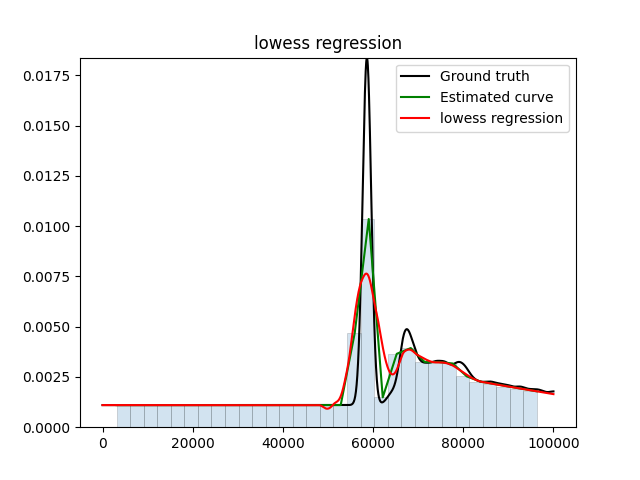
\includegraphics[width=\linewidth]{lowess_ewh_graph}
\caption{EWH}
\end{subfigure}
\hfill
\begin{subfigure}[h]{0.5\linewidth}
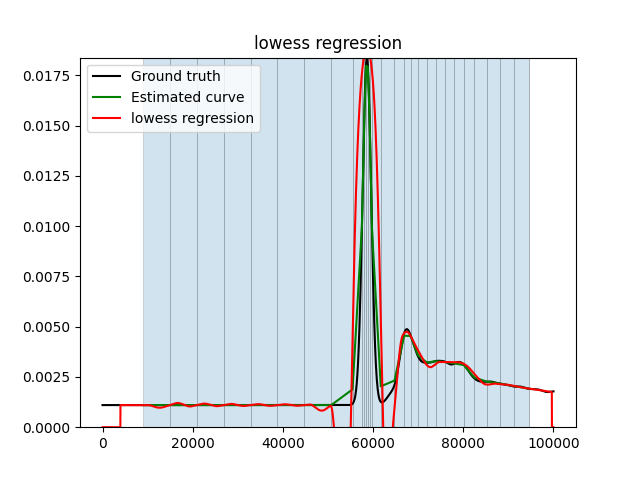
\includegraphics[width=\linewidth]{lowess_edh_graph}
\caption{EDH}
\end{subfigure}
\caption{Lowess regression plotted against EW \& ED datasets}
\end{figure}
As shown in the figure, for both the equi-width and equi-depth datasets, the regression model does
a rather good job at modelling the distribution. However, there are some rather noticable flaws.
In the equi-width data the model fails to overfit the datapoints and such has a large error
between the local maximums of both the estimated and ground-truth datasets. In the equi-depth
data the model ends up overfitting slightly and creating un-realistic dips below zero near large
changes in slope. 
\begin{figure}[H]
\centering
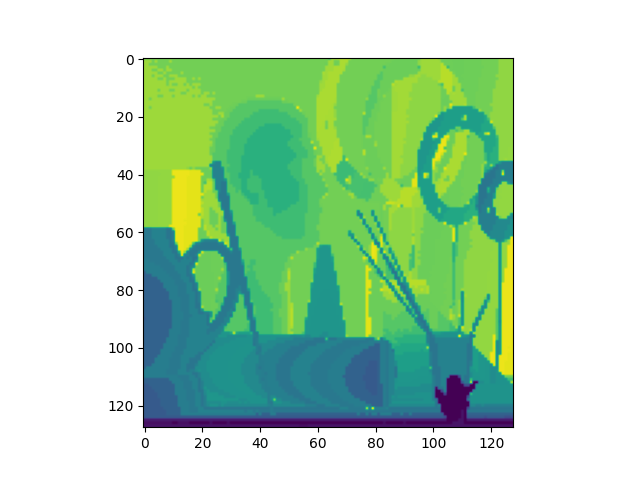
\includegraphics{lowess_depthmap}
\caption{Depthmap using Lowess regression}
\end{figure}
Looking at the depth map in \emph{figure 2}, lowess regression does suceed rather well at 
recreating the depth of the image, even going as far as providing more depth details
in some areas compared to the equi-depth data. However, some oversaturation and noise is caused
due to the overfitting of the regression model on the equi-depth data.

\subsection{Method 2: Gaussian Process Regression}
Gaussian Process (GP) regression is another non-parametic regression method that, in simplest
form, attempts to find the most accurate function over a variety of different potential functions.
This is done through the use of a kernel function to find the covariance between each point, which
can then be compared with each of the potential functions to identify the best fit 
(\cite{wang2020intuitive}). Knowledge of the specifics of how GP works is not the focus of
this paper and is not required for testing it's usefulness as a regression method. One of
the most important aspects that does need to carefully considered, however is the kernel 
function used, as it ultimately defines the smoothness and fitting of the predicted function.
The most commonly used kernel, due to it's "universal" properties and simplicity, is the
Radial Basis Function (RBF) kernel (also known as the Squared Exponential kernel or Gaussian
kernel), and can be defined as: (equation goes here) where $l$ is the "lengthscale", aka the
maximum distance where two points are considered "similar" and not outliers (\cite{Duvenaud}). 
an easy method for finding the length scale that best fits our dataset would be to find the 
mean difference between each $x$ point, and while this would work for the equi-width data,
it would have much less effectiveness with the equi-depth datapoints as the differences between 
points convulge at the peak of the laser thus skewing the mean. This lead to us using the 
Rational Quadratic (RQ) function as our kernel function. The RQ function is rather similar in 
both form and functionality to the RBF, with the difference of taking on an extra parameter 
$\alpha$, which determines the possible variation $l$ can adjust to. 
\begin{figure}[H]
\begin{subfigure}[h]{0.5\linewidth}
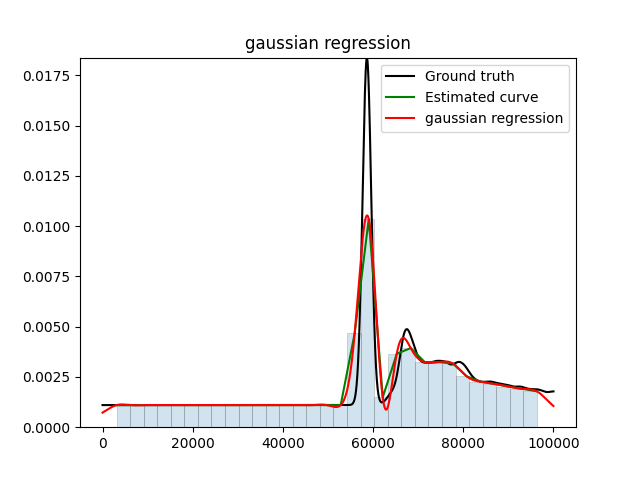
\includegraphics[width=\linewidth]{gaussian_ewh_graph}
\caption{EWH}
\end{subfigure}
\hfill
\begin{subfigure}[h]{0.5\linewidth}
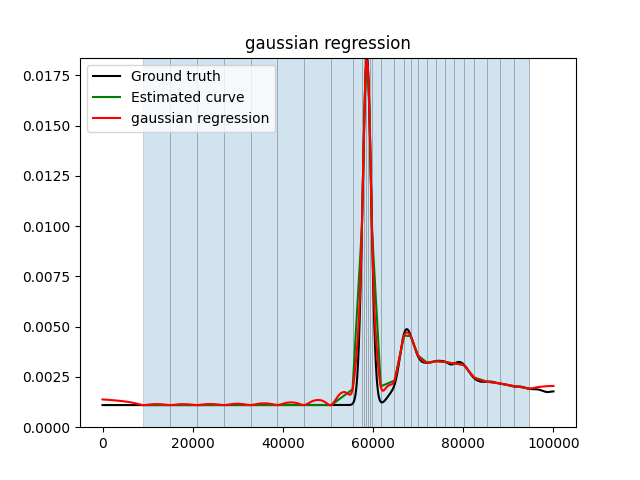
\includegraphics[width=\linewidth]{gaussian_edh_graph}
\caption{EDH}
\end{subfigure}
\caption{Gaussian Process regression plotted against EW \& ED datasets}
\end{figure}
This kernel function ends up working much better for both the equi-width and equi-depth datasets, 
as seen in \emph{figure 3}, as we can set $\alpha$ to be the ratio of the minimum difference of 
$x$ over the maximum difference of $x$ to allow for variations in fitting throughout the 
response curve. Both scikit learn's \verb|GaussianProcessorRegressor()| and 
\verb|RationalQuadratic()| classes were used in order to easily test this regression in python 
(\cite{scikit-learn}). This ends up giving a incredibly smooth resoponse curve that closely 
matches the local maximum of the ground-truth data. The depth map shown in \emph{figure 4} 
is also impressive, again minus some points of oversaturation caused by overfitting.
\begin{figure}[H]
\centering
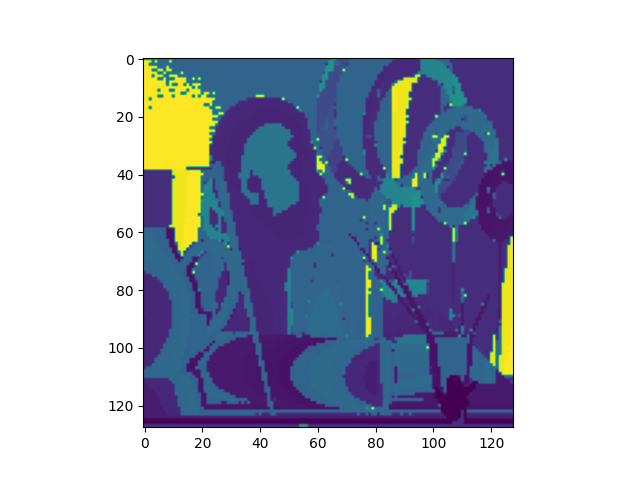
\includegraphics{gaussian_depthmap}
\caption{Depthmap using Gaussian Process regression}
\end{figure}

\subsection{Method 3: Kernel Density Estimation}
Another way we can look at this problem is instead of estimating a curve for photon intensity
over exposure time, we can observe the photon response curve as a measure of the probability of 
photon readings over exposure time. This would allow for us to use Kernel Density Estimation (KDE)
to estimate the probability density function of the data, which can then scaled to fit the 
original photon intensity data. The KDE function can be defined as (equation goes here) where
$K()$ is a kernel function passed (\cite{chen2018lecture}). Unlike in GP regression, the 
objective of the kernel function is to determine the weight of the point based on the number 
of points under the function's curve. $h$ is the bandwidth which, similar to the lengthscale 
in an RBF, defines the smoothness and fitting. we ended up using scipy's \verb|gaussian_kde()| 
class to implement this method (\cite{virtanen2020scipy}), mainly due to it's ease of use 
and higher performance for smaller datasets (\cite{VanderPlas_2023}). The bandwidth for the
model was set to $0.05$ (or rather $0.05$ multiplied by the standard deviation due to how
the class works) in order to allow for some overfitting, again due to the limited set.
\begin{figure}[H]
\centering
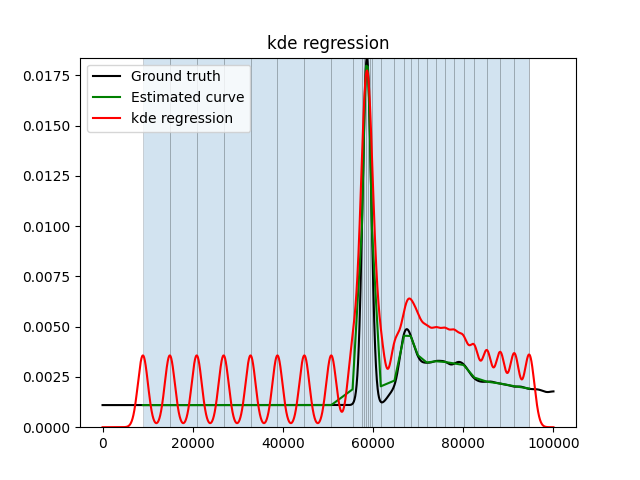
\includegraphics[width=\linewidth]{kde_edh_graph}
\caption{Kernel Density Estimation plotted against ED dataset}
\end{figure}
The equi-depth graph shown in \emph{figure 5} shows a decent attempt of modeling the response
curve, with the smoothness of the model being mostly accurate outside of the high amounts
of "wiggly" fits where ambient light should be. One important thing to mention is that 
KDE can't be used for the equi-width dataset without heavy modification, as all the points
arrive at equal intervals. Looking at the depth map in \emph{figure 6}, while their is a lot
less oversaturation, the model fails to model as much depth compared to either LOWESS or GP.
\begin{figure}[H]
\centering
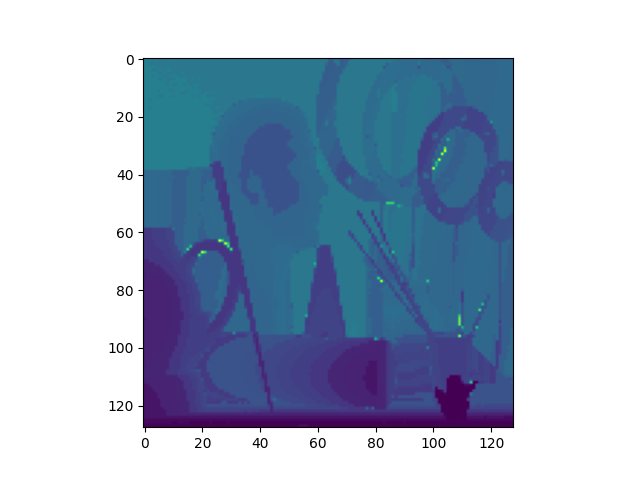
\includegraphics{kde_depthmap}
\caption{Depthmap using Kernel Density Estimation}
\end{figure}

\section{Results}
Along with comparing the graphs of each regression method against the ground-truth data,
error statistics were also calculated for both equi-width and equi-depth in order to 
have quantitative data to make comparisons. Four statistics were calculated with help of
scikit learn's regression error functions (\cite{scikit-learn}): coefficient of determination
($R^2$), mean squared error (MSE), max value error, and peak error. 
\begin{table}[H]
\centering
\resizebox{\textwidth}{!}{
\begin{tabular}{l|l|l|}
\cline{2-3}
                                                        & gaussian               & lowess                 \\ \hline
\multicolumn{1}{|l|}{Coefficient of Determination (R2)} & 0.8009545141717576     & 0.6030621202394134     \\ \hline
\multicolumn{1}{|l|}{Mean Squared Error}                & 1.0425674355239912e-06 & 2.0790951658226772e-06 \\ \hline
\multicolumn{1}{|l|}{Max Error}                         & 0.007852506269561368   & 0.010754308473284957   \\ \hline
\multicolumn{1}{|l|}{Peak Error}                        & 0.007850089280617817   & 0.010744692981616531   \\ \hline
\end{tabular}
}
\caption{Error statistics for EWH}
\end{table}
Looking at the equi-width statistics in \emph{table 1}, we can see that, although not 
by a large margin, GP had better quantitative results than LOWESS. Similarly, in 
\emph{table 2}, we can see this lead improve by a larger margin, even when compared to KDE. 
In fact, LOWESS's $R^2$ actually fell below zero, and had a much higher error stats due to 
the large dips below zero at each large change in slope. If a method had been implemented to 
prevent LOWESS from falling below zero, it might have been a much less computationally expensive 
alternative to GP regression.
\begin{table}[H]
\centering
\resizebox{\textwidth}{!}{
\begin{tabular}{l|l|l|l|}
\cline{2-4}
                                                        & gaussian               & lowess                & kde                   \\ \hline
\multicolumn{1}{|l|}{R2}                                & 0.984733622701605      & -0.015483069257797633 & 0.46294427914834313   \\ \hline
\multicolumn{1}{|l|}{Mean Squared Error}                & 7.996276712079517e-08  & 5.318932880737122e-06 & 2.81300931438835e-06  \\ \hline
\multicolumn{1}{|l|}{Max Error}                         & 0.0015863146232056053  & 0.011393197052572267  & 0.0052443981426180215 \\ \hline
\multicolumn{1}{|l|}{Peak Error}                        & 0.00013488165733672314 & 0.0004277378621173611 & 0.0006406705077052141 \\ \hline
\end{tabular}
}
\caption{Error statistics for EDH}
\end{table}

\section{Conclusion}
Overall, each of the three non-parametic regression models tested in this experiment succedded 
in being able model the distribution of a photon arrival time response curve. Both quantitatively
and visually, GP regression was the strongest model. However due to it's complexity, specifically 
computationally, it might be more efficient to use lowess regression and smooth out any dips 
below zero in order to avoid turning a data transfer problem into a computational problem. One
important thing to note is that there are a variety of improvements that can be made on the models
tested, especially with KDE. GP regression could have implemented an original kernel function
tailored to this specific problem, and LOWESS regression could have as stated prior implemented
a method to follow the rules of poisson statistics. Most drastically, KDE could have made use
of an actual method (such as Silverman's rule of Cross examination) in order to have a variable
bandwidth per pixel analyzed, which might have made it a more viable option. Regardless, all
three methods have shown a future of being able to model photon arrival response curves using
regression, which not only helps with reducing the amount of data needing be collected by the
camera but also providing more qualitative data that can be used to optimize imaging of
single-photon 3D cameras even further.

\section{Acknowledgements}
Thank you to Kaustubh Sadekar and the rest of 
\href{https://www.computational.camera/team}{PSU's Computational Imaging Lab Team} for providing
both code and educational resources. Huge thank you to my mentor Daphne Kurzenhauser for guiding 
and advising me throughout the course of this research project.

\printbibliography
\end{document}
